\subsection{\gls{crna} annotation}
In its minimal form, a \gls{crna} is defined by the chromosome it is located on
and the start and end position of the \gls{bsj}.
While this information is sufficient to uniquely identify a \gls{bsj}, it does
not provide any information about the gene or genes it is part of.
Furthermore, it does not give any information about the type of \gls{crna} it
is (types of \gls{crna} are described in \cref{sec:circrna_types}) and if it is
already has an entry in any \gls{crna} database.
While some tools like CircExplorer2 and DCC provide their own annotation, other
tools like find\_circ and segemehl do not.
To provide a consistent annotation for all \glspl{bsj}, nf-core/circrna uses a
custom annotation process that will be described in the following sections.

\subsubsection{\gls{gtf} based annotation}
\gls{gtf} files are a common way to store genomic annotations like gene
locations and
transcript structures.
Such files are available for many reference genomes and can be used to identify
the genes and linear transcripts a \gls{crna} overlaps with.
This information can be used to infer the host gene(s) and the type of
\gls{crna}.

\begin{figure}[ht]
    \centering

    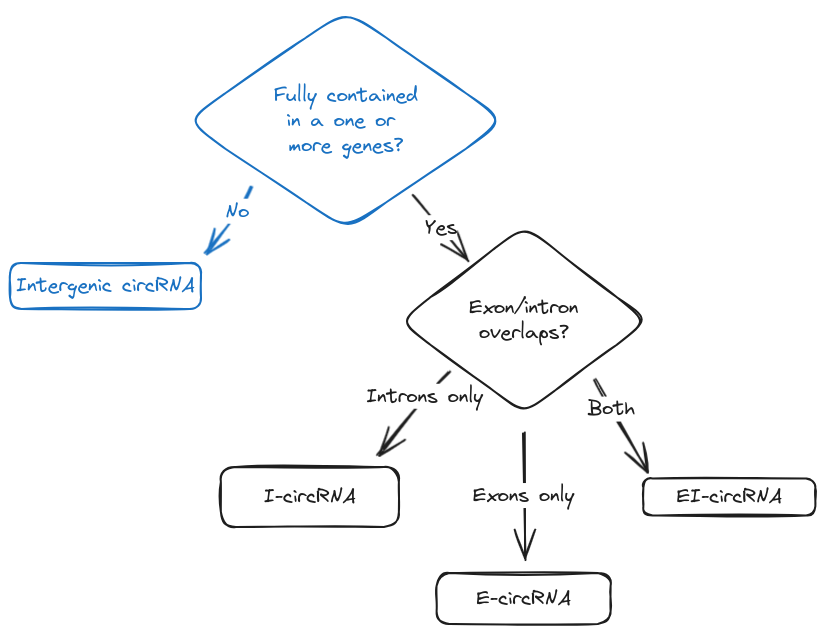
\includegraphics[width=\textwidth]{chapters/3_materials_and_methods/figures/annotation.png}
    \caption{\gls{gtf} annotation workflow} % TODO: Add detailed caption
    \label{fig:gtf_annotation}
\end{figure}

The nf-core/circrna pipeline approaches this as shown in
\cref{fig:gtf_annotation}: \begin{enumerate} \item If the \gls{crna} does not
          overlap with any gene, it is labeled as \gls{ig-crna}.
    \item If the \gls{crna} overlaps with at least one gene, but is not fully
          contained by any gene, it is labeled as \gls{pig-crna}.
    \item If the \gls{crna} is fully contained in any gene, the following
          classification is performed:
          \begin{itemize}
              \item If the \gls{crna} is fully contained in an exon, it is
                    labeled as \gls{e-crna}.
              \item If the \gls{crna} is fully contained in an intron, it is
                    labeled as \gls{i-crna}.
              \item If the \gls{crna} spans both exonic and intronic regions,
                    it is labeled as \gls{ei-crna}.
          \end{itemize}
\end{enumerate}

\subsubsection{Database based annotation} Describe database based annotation